\documentclass[journal]{IEEEtran}

% ============================================================
% PACKAGES
% ============================================================
\usepackage{amsmath,amssymb}
\usepackage{graphicx}
\usepackage{booktabs}
\usepackage{multirow}
\usepackage{siunitx}
\usepackage{cite}
\usepackage{url}
\usepackage{xcolor}
\usepackage{bm}

% ============================================================
% FIGURE PATHS
% ============================================================
\graphicspath{
	{../figures/Whakaari_2019/}
}

% ============================================================
% SI UNIT SETUP
% ============================================================
\sisetup{
	scientific-notation = true,
	round-mode = places,
	round-precision = 2
}

% ============================================================
% TITLE
% ============================================================

\title{
	Multi-Scale Ordinal-Pattern Entropy--Complexity Analysis 
	of RSAM Data From the 2019 Whakaari Eruption
}

% ============================================================
% AUTHORS
% ============================================================

\author{
	Rasika Dilhani,
	Alejandro C. Frery,
	Andrea Rey,
	and~[Other Authors]
	%
	\thanks{
		R. Dilhani is with the School of Mathematics and Statistics,
		Victoria University of Wellington, Wellington, New Zealand.
	}
}

\begin{document}
	
	\maketitle
	
	% ============================================================
	% ABSTRACT
	% ============================================================
	
	\begin{abstract}
		
		Real-time Seismic Amplitude Measurement (RSAM) provides a
		continuous representation of volcanic seismic activity and is
		widely used for monitoring changes in volcanic systems.
		This study investigates whether ordinal-pattern-based
		information-theoretic measures can characterize changes in RSAM
		dynamics associated with the 9 December 2019 eruption of Whakaari
		(White Island), New Zealand.
		
		Continuous RSAM observations recorded at the WIZ seismic station
		were analysed using ordinal pattern probability distributions and
		four complementary information-theoretic frameworks: Shannon
		entropy, R\'enyi entropy, Tsallis entropy, and the Fisher
		Information Measure, together with their corresponding statistical
		complexity measures.
		
		A multi-scale temporal analysis was performed. Weekly RSAM
		segments were analysed using embedding dimension $D=5$, while
		daily segments were analysed using $D=3$ to account for the
		smaller number of observations available within each daily
		window. The resulting entropy--complexity representations were
		used to investigate changes in seismic dynamics throughout 2019.
		
		The weekly analysis identified distinct changes in the
		entropy--complexity plane during the period immediately preceding
		and containing the December 2019 eruption. The daily analysis
		provided finer temporal localization and independently identified
		the eruption-associated period as exhibiting dynamics distinct
		from background seismic behaviour. The consistency of the
		signatures across temporal scales indicates that ordinal-pattern
		information-theoretic measures are sensitive to changes in the
		temporal organization of volcanic seismic signals.
		
		These results demonstrate the potential of entropy--complexity
		analysis as a complementary approach for characterizing volcanic
		seismic dynamics from continuous RSAM observations.
		
	\end{abstract}
	
	% ============================================================
	% KEYWORDS
	% ============================================================
	
	\begin{IEEEkeywords}
		Whakaari, volcanic seismicity, RSAM, ordinal patterns,
		permutation entropy, statistical complexity,
		Fisher information, eruption monitoring.
	\end{IEEEkeywords}
	
	
	% ============================================================
	\section{Introduction}
	% ============================================================
	
	\IEEEPARstart{V}{olcanic} eruptions represent a major natural
	hazard and may produce severe impacts on communities,
	infrastructure, aviation, and the environment.
	
	% ------------------------------------------------------------
	% Suggested order:
	%
	% Paragraph 1: Volcano monitoring problem
	% Paragraph 2: Whakaari and 2019 eruption
	% Paragraph 3: RSAM
	% Paragraph 4: Information-theoretic approaches
	% Paragraph 5: Ordinal patterns
	% Paragraph 6: Research gap
	% Paragraph 7: Contributions
	% ------------------------------------------------------------
	
	Volcanic seismic monitoring provides continuous information
	regarding changes within active volcanic systems. Among the
	quantities commonly used for operational monitoring, Real-time
	Seismic Amplitude Measurement (RSAM) provides a computationally
	efficient summary of seismic amplitude and has been widely
	employed to characterize volcanic unrest \cite{Endo1991}.
	
	Information-theoretic approaches provide an alternative means of
	characterizing seismic signals by quantifying their temporal
	organization rather than considering amplitude alone.
	Previous investigations have demonstrated the usefulness of
	entropy and Fisher-information-based measures for identifying
	changes associated with volcanic activity
	\cite{Telesca2014,ReyDevesa2023}.
	
	Ordinal patterns provide a particularly attractive representation
	for this purpose because they describe the relative temporal
	ordering of observations rather than their absolute amplitudes
	\cite{Bandt2002}.
	
	Despite their application to several nonlinear time-series
	problems, the potential of ordinal-pattern-based entropy and
	complexity measures for analysing continuous RSAM observations
	from Whakaari remains comparatively unexplored.
	
	The objective of this study is therefore to investigate whether
	ordinal-pattern information-theoretic descriptors can identify
	changes in the temporal dynamics of RSAM associated with the
	9 December 2019 Whakaari eruption.
	
	The main contributions of this work are:
	
	\begin{enumerate}
		\item development of an ordinal-pattern representation of
		continuous RSAM observations;
		
		\item comparison of Shannon, R\'enyi, Tsallis, and Fisher
		information-theoretic representations;
		
		\item investigation of the 2019 seismic dynamics using
		weekly windows with embedding dimension $D=5$;
		
		\item refinement of the analysis to daily resolution using
		embedding dimension $D=3$; and
		
		\item evaluation of the consistency of eruption-associated
		signatures across multiple temporal resolutions.
	\end{enumerate}
	
	
	% ============================================================
	\section{Study Area and Data}
	% ============================================================
	
	\subsection{Whakaari and the WIZ Seismic Station}
	
	Whakaari (White Island) is an active volcanic system located
	offshore from the eastern coast of New Zealand's North Island.
	
	% Add geological/monitoring context here.
	
	\begin{figure}[!t]
		\centering
		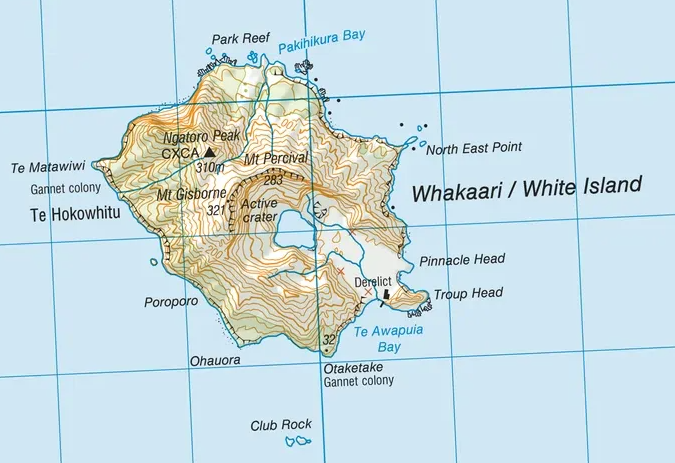
\includegraphics[width=\columnwidth]{Whakaari}
		\caption{
			Location of the WIZ seismic station on Whakaari
			(White Island), New Zealand.
		}
		\label{fig:study_area}
	\end{figure}
	
	
	\subsection{RSAM Data}
	
	The dataset consists of continuous seismic amplitude observations
	recorded at the WIZ seismic station.
	
	The original waveform was sampled at \SI{100}{Hz}. For the present
	analysis, RSAM observations averaged over non-overlapping
	10-minute intervals were used.
	
	A complete day therefore contains approximately
	
	\begin{equation}
		N_{\mathrm{day}} = 24 \times 6 = 144
	\end{equation}
	
	observations, while a complete seven-day interval contains
	
	\begin{equation}
		N_{\mathrm{week}} = 7 \times 144 = 1008
	\end{equation}
	
	observations.
	
	
	\subsection{The 2019 Whakaari Eruption}
	
	The principal event considered in this study is the eruption of
	Whakaari on 9 December 2019.
	
	% Describe eruption time and monitoring context here.
	
	
	% ============================================================
	\section{Methodology}
	% ============================================================
	
	\subsection{Ordinal Pattern Representation}
	
	Consider a time series
	
	\begin{equation}
		X = \{x_t\}_{t=1}^{N}.
	\end{equation}
	
	For embedding dimension $D$ and time delay $\tau$, each
	embedding vector is defined as
	
	\begin{equation}
		\mathbf{x}_t =
		(x_t,x_{t+\tau},\ldots,x_{t+(D-1)\tau}).
	\end{equation}
	
	The relative ordering of the components of $\mathbf{x}_t$
	defines an ordinal pattern
	
	\begin{equation}
		\pi_t \in S_D,
	\end{equation}
	
	where $S_D$ denotes the set of all $D!$ possible permutations.
	
	The empirical probability associated with pattern $\pi_i$ is
	
	\begin{equation}
		p_i =
		\frac{n_i}
		{N-(D-1)\tau},
	\end{equation}
	
	where $n_i$ denotes the number of occurrences of the $i$th
	ordinal pattern.
	
	The resulting probability vector is
	
	\begin{equation}
		\mathbf{P} =
		(p_1,p_2,\ldots,p_{D!}).
	\end{equation}
	
	
	% ============================================================
	\subsection{Shannon Permutation Entropy}
	
	The normalized Shannon entropy is
	
	\begin{equation}
		H_S(\mathbf{P})
		=
		-\frac{1}{\ln(D!)}
		\sum_{i=1}^{D!}
		p_i \ln p_i.
		\label{eq:shannon}
	\end{equation}
	
	It satisfies
	
	\begin{equation}
		0 \le H_S \le 1.
	\end{equation}
	
	
	% ============================================================
	\subsection{R\'enyi Entropy}
	
	For $q>0$, $q\neq1$, the normalized R\'enyi entropy is
	
	\begin{equation}
		H_R^{(q)}(\mathbf{P})
		=
		\frac{
			\ln\left(
			\sum_{i=1}^{D!}p_i^q
			\right)
		}{
			(1-q)\ln(D!)
		}.
	\end{equation}
	
	
	% ============================================================
	\subsection{Tsallis Entropy}
	
	For $q\neq1$, Tsallis entropy is
	
	\begin{equation}
		S_T^{(q)}(\mathbf{P})
		=
		\frac{
			1-\sum_{i=1}^{D!}p_i^q
		}{
			q-1
		}.
	\end{equation}
	
	Its normalized form is denoted by
	
	\begin{equation}
		H_T^{(q)}(\mathbf{P}).
	\end{equation}
	
	
	% ============================================================
	\subsection{Fisher Information Measure}
	
	The discrete Fisher Information Measure is defined as
	
	\begin{equation}
		F(\mathbf{P})
		=
		4
		\sum_{i=1}^{D!-1}
		\left(
		\sqrt{p_{i+1}}
		-
		\sqrt{p_i}
		\right)^2.
		\label{eq:fisher}
	\end{equation}
	
	
	% ============================================================
	\subsection{Disequilibrium and Statistical Complexity}
	
	Let
	
	\begin{equation}
		\mathbf{P}_e =
		\left(
		\frac{1}{D!},\ldots,\frac{1}{D!}
		\right)
	\end{equation}
	
	denote the uniform distribution.
	
	The Jensen--Shannon divergence between $\mathbf{P}$ and
	$\mathbf{P}_e$ is
	
	\begin{equation}
		J(\mathbf{P},\mathbf{P}_e)
		=
		S\left(
		\frac{\mathbf{P}+\mathbf{P}_e}{2}
		\right)
		-
		\frac{1}{2}S(\mathbf{P})
		-
		\frac{1}{2}S(\mathbf{P}_e).
	\end{equation}
	
	The normalized disequilibrium is
	
	\begin{equation}
		Q_J(\mathbf{P},\mathbf{P}_e)
		=
		Q_0
		J(\mathbf{P},\mathbf{P}_e),
	\end{equation}
	
	where $Q_0$ is a normalization constant.
	
	The Shannon statistical complexity is then
	
	\begin{equation}
		C_S
		=
		H_S Q_J.
	\end{equation}
	
	Analogously,
	
	\begin{equation}
		C_R = H_R Q_J,
	\end{equation}
	
	\begin{equation}
		C_T = H_T Q_J,
	\end{equation}
	
	and the Fisher-based complexity is
	
	\begin{equation}
		C_F = F Q_J.
	\end{equation}
	
	
	% ============================================================
	\subsection{Multi-Scale Experimental Design}
	% ============================================================
	
	The analysis was performed at multiple temporal resolutions to
	investigate whether eruption-associated changes were preserved
	when the duration of the analysis window was reduced.
	
	
	\subsubsection{Monthly Analysis}
	
	The 2019 RSAM record was initially divided according to calendar
	month. Ordinal-pattern entropy and complexity measures were
	computed for each month to provide a coarse-scale representation
	of the temporal evolution of the seismic signal.
	
	
	\subsubsection{Weekly Analysis}
	
	For the weekly experiment, the 10-minute RSAM series was
	partitioned into seven-day windows.
	
	Successive windows were shifted by six days, resulting in a
	one-day overlap between consecutive windows.
	
	Each complete weekly segment contained approximately 1008
	observations.
	
	Ordinal patterns were generated using
	
	\begin{equation}
		D=5,
		\qquad
		\tau=1.
	\end{equation}
	
	The number of possible ordinal patterns is therefore
	
	\begin{equation}
		D! = 5! = 120.
	\end{equation}
	
	
	\subsubsection{Daily Analysis}
	
	To obtain finer temporal localization, the 2019 RSAM record was
	subsequently analysed using daily windows.
	
	Each complete daily interval contains approximately 144
	10-minute RSAM observations.
	
	For the daily analysis, the embedding parameters were
	
	\begin{equation}
		D=3,
		\qquad
		\tau=1,
	\end{equation}
	
	corresponding to
	
	\begin{equation}
		D! = 3! = 6
	\end{equation}
	
	possible ordinal patterns.
	
	The lower embedding dimension was selected because the shorter
	daily windows contain substantially fewer observations than the
	weekly windows. Using $D=5$ would require estimating probabilities
	for 120 possible ordinal patterns from approximately 140 embedded
	vectors, resulting in sparse probability estimates. In contrast,
	$D=3$ provides six possible patterns and therefore permits more
	stable estimation of the ordinal-pattern distribution within each
	daily segment.
	
	
	% ============================================================
	\section{Results}
	% ============================================================
	
	\subsection{Exploratory Analysis of RSAM}
	
	% Put annual statistics and violin plot here.
	% Keep this subsection SHORT in the journal paper.
	
	
	\subsection{Monthly Entropy--Complexity Representation}
	
	Figure~\ref{fig:monthly_hc} presents the monthly
	entropy--complexity representation for 2019.
	
	\begin{figure}[!t]
		\centering
		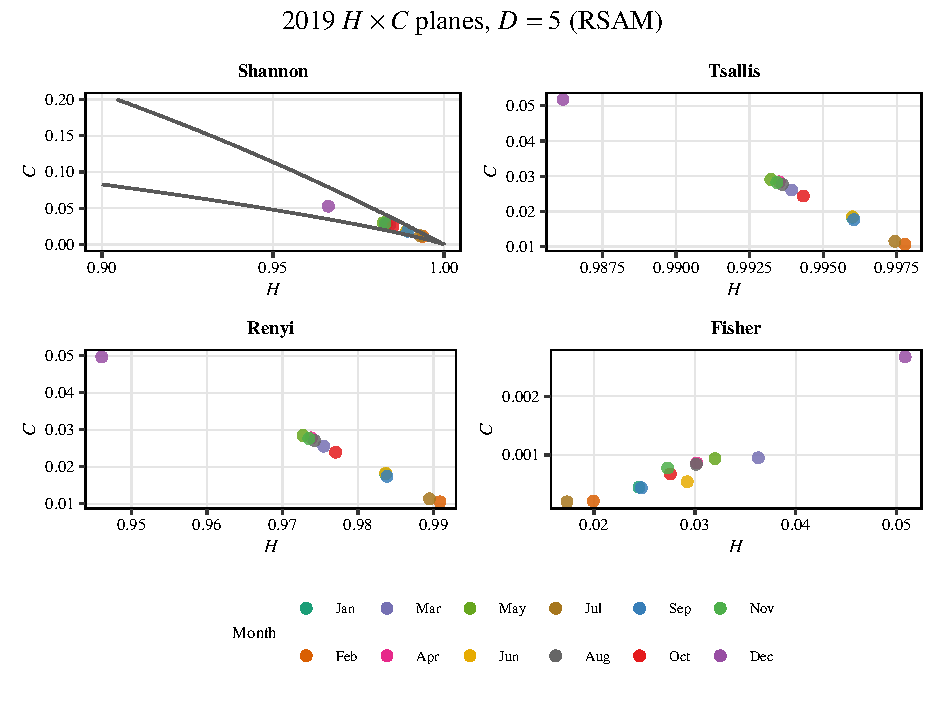
\includegraphics[width=\columnwidth]
		{HC_Combined_2019_RSAM_D5_Months_No_CI}
		\caption{
			Monthly entropy--complexity representations of the 2019
			RSAM time series.
		}
		\label{fig:monthly_hc}
	\end{figure}
	
	
	% ============================================================
	\subsection{Weekly Entropy--Complexity Analysis}
	% ============================================================
	
	The weekly analysis provides a finer representation of the
	temporal evolution of seismic dynamics during 2019.
	
	\begin{figure*}[!t]
		\centering
		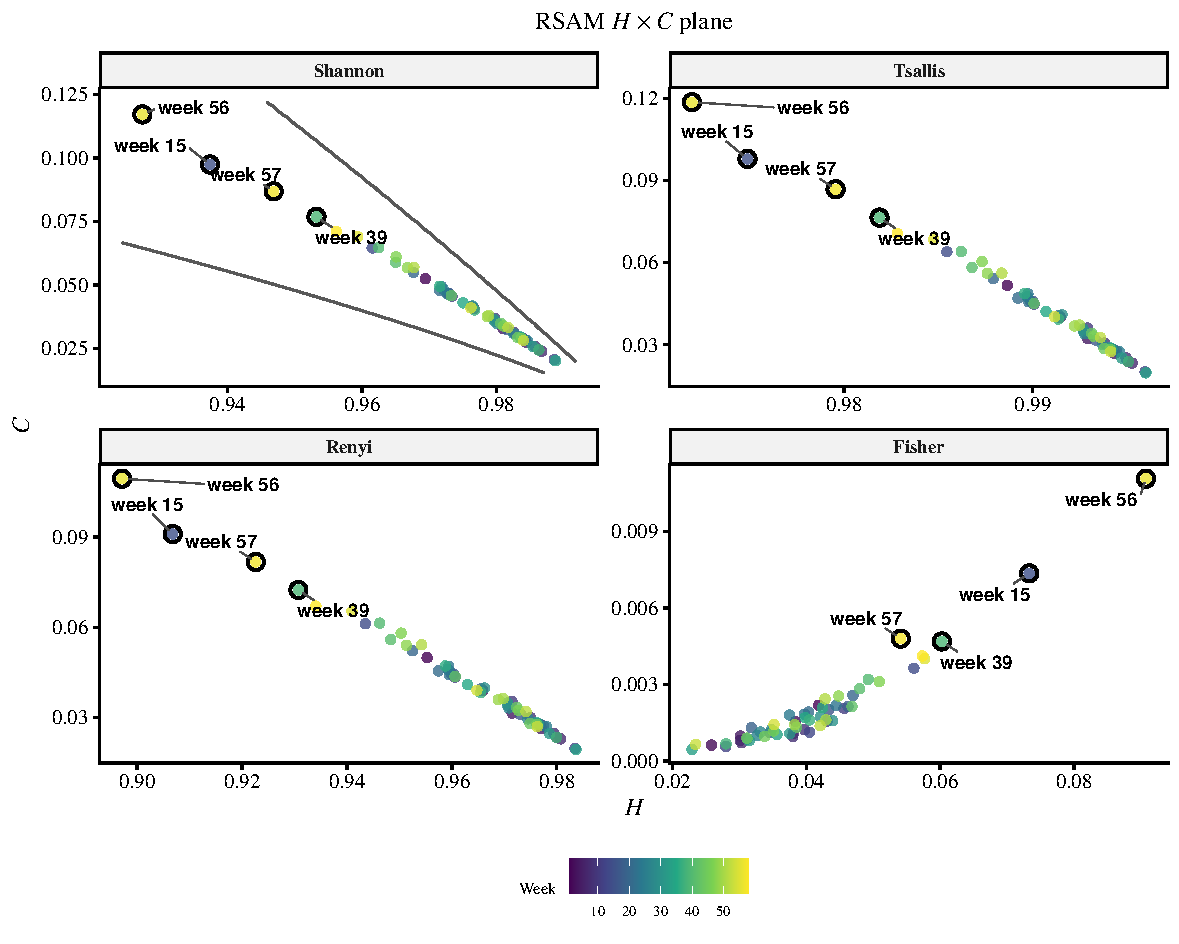
\includegraphics[width=0.95\textwidth]
		{HC_Plane_rsam_avg_D5_noCI_upto9Dec}
		\caption{
			Weekly entropy--complexity representation of the 2019 RSAM
			observations using $D=5$ and $\tau=1$.
		}
		\label{fig:weekly_hc}
	\end{figure*}
	
	The Shannon-, R\'enyi-, and Tsallis-based representations show
	that several weeks immediately preceding the 9 December eruption
	occupy extreme regions of the entropy--complexity plane.
	
	In particular, Week~56 exhibits the lowest entropy and largest
	complexity values among the analysed weekly segments, while
	Week~57, which includes the eruption period, also exhibits a
	distinct entropy--complexity signature.
	
	% Your table of extreme weeks goes here.
	
	
	% ============================================================
	\subsection{Daily Entropy--Complexity Analysis}
	% ============================================================
	
	The daily analysis was performed to determine whether the
	eruption-associated behaviour observed at weekly resolution could
	be localized more precisely in time.
	
	Each point in Fig.~\ref{fig:daily_hc} represents the ordinal
	pattern distribution obtained from one day of RSAM measurements.
	
	\begin{figure*}[!t]
		\centering
		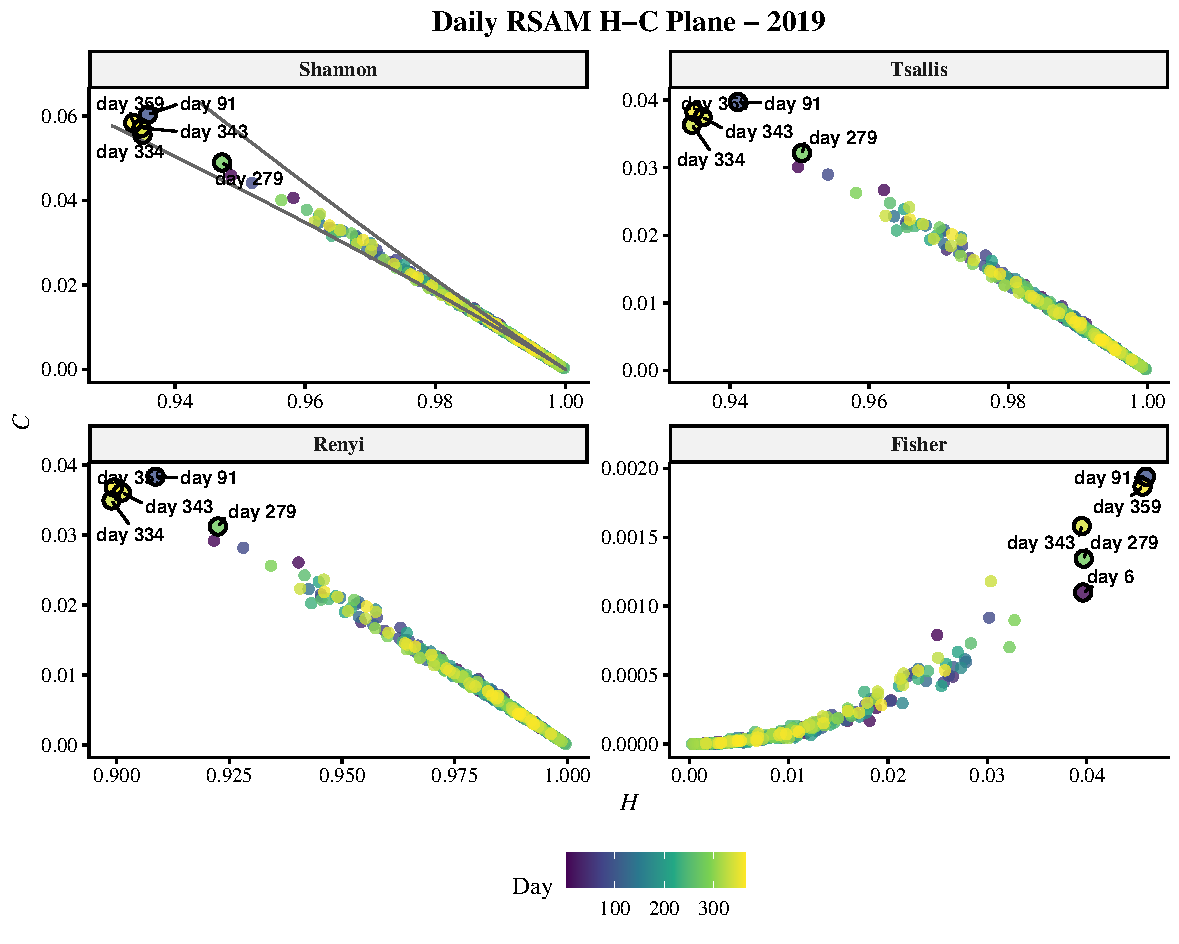
\includegraphics[width=0.95\textwidth]
		{HC_Plane_RSAM_D3_noCI}
		\caption{
			Daily entropy--complexity representations of the 2019 RSAM
			time series obtained using embedding dimension $D=3$ and
			time delay $\tau=1$.
		}
		\label{fig:daily_hc}
	\end{figure*}
	
	The day associated with the 9 December 2019 eruption occupies an
	extreme region of the entropy--complexity plane relative to
	background days.
	
	% Insert your exact daily results here.
	%
	% Example:
	%
	% The eruption day exhibited ...
	% Shannon H = ...
	% Shannon C = ...
	% etc.
	
	
	% ============================================================
	\subsection{Comparison Across Temporal Scales}
	% ============================================================
	
	The monthly, weekly, and daily analyses show a progressive
	localization of the anomalous seismic dynamics associated with
	the December 2019 eruptive episode.
	
	At monthly resolution, December is distinguishable from the
	remaining months of 2019. At weekly resolution, the analysis
	identifies unusual dynamics during the weeks immediately
	preceding and containing the eruption. At daily resolution, the
	anomalous behaviour is localized more precisely to the
	eruption-associated period.
	
	The persistence of the entropy--complexity signature across
	multiple temporal resolutions indicates that the observed
	departure from background behaviour is not solely a consequence
	of a particular window size.
	
	
	% ============================================================
	\subsection{Multivariate Feature Analysis}
	% ============================================================
	
	% OPTIONAL SECTION
	%
	% Correlation
	% PCA
	% DBSCAN
	%
	% Keep this shorter than in your present report unless the
	% clustering becomes a major contribution.
	
	
	% ============================================================
	\section{Discussion}
	% ============================================================
	
	The results demonstrate that ordinal-pattern-based
	information-theoretic measures capture changes in the temporal
	organization of the Whakaari RSAM signal associated with the
	December 2019 eruptive episode.
	
	\subsection{Weekly Pre-Eruption Signature}
	
	% Discuss Weeks 56 and 57.
	% Do NOT call it forecasting unless evidence supports forecasting.
	
	
	\subsection{Daily Localization of the Eruption}
	
	% Explain how the daily D=3 analysis sharpens temporal resolution.
	
	
	\subsection{Agreement Among Information-Theoretic Measures}
	
	% Shannon
	% Renyi
	% Tsallis
	% Fisher
	
	
	\subsection{Effect of Temporal Resolution and Embedding Dimension}
	
	The use of different embedding dimensions at weekly and daily
	scales reflects the trade-off between ordinal-pattern resolution
	and the number of observations available for estimating pattern
	probabilities.
	
	% Develop this argument.
	
	
	\subsection{Relation to Previous Volcanic Seismic Studies}
	
	% Compare with Telesca
	% Rey-Devesa
	% Dempsey
	% etc.
	
	
	\subsection{Limitations}
	
	Several limitations should be considered.
	
	First, the analysis focuses primarily on the 2019 eruptive
	episode and therefore does not establish that the identified
	signatures constitute general eruption precursors.
	
	Second, entropy--complexity anomalies may also occur during
	non-eruptive periods of volcanic unrest.
	
	Third, the ordinal-pattern probability estimates depend on the
	selected temporal window, embedding dimension, and time delay.
	
	Consequently, the present results should be interpreted as a
	characterization of changes in seismic dynamics rather than as
	an eruption forecasting model.
	
	
	% ============================================================
	\section{Conclusion}
	% ============================================================
	
	This study investigated the use of ordinal-pattern-based
	information-theoretic measures for characterizing RSAM dynamics
	associated with the 2019 Whakaari eruption.
	
	Analysis at weekly resolution using embedding dimension $D=5$
	identified distinct entropy--complexity behaviour immediately
	before and during the December 2019 eruptive period.
	
	A complementary daily analysis using $D=3$ reproduced the
	eruption-associated signature at a finer temporal resolution.
	
	The agreement between the weekly and daily analyses demonstrates
	that changes in the temporal ordering of RSAM observations are
	detectable across multiple temporal scales.
	
	These findings suggest that ordinal-pattern entropy and
	statistical complexity provide useful complementary descriptors
	for investigating changes in volcanic seismic dynamics.
	
	Future work will evaluate the stability of these signatures
	across additional eruptive and non-eruptive periods and examine
	their relationship with independent indicators of volcanic
	unrest.
	
	
	% ============================================================
	% REFERENCES
	% ============================================================
	
	\bibliographystyle{IEEEtran}
	\bibliography{seismic_references}
	
\end{document}